\documentclass[a4paper,twoside]{article}
\usepackage[T1]{fontenc}
\usepackage[bahasa]{babel}
\usepackage{graphicx}
\usepackage{graphics}
\usepackage{float}
\usepackage[cm]{fullpage}
\pagestyle{myheadings}
\usepackage{etoolbox}
\usepackage{setspace} 
\usepackage{lipsum} 
\setlength{\headsep}{30pt}
\usepackage[inner=2cm,outer=2.5cm,top=2.5cm,bottom=2cm]{geometry} %margin
% \pagestyle{empty}
\usepackage{booktabs}

\makeatletter
\renewcommand{\@maketitle} {\begin{center} {\LARGE \textbf{ \textsc{\@title}} \par} \bigskip {\large \textbf{\textsc{\@author}} }\end{center} }
\renewcommand{\thispagestyle}[1]{}
\markright{\textbf{\textsc{Laporan Perkembangan Pengerjaan Skripsi\textemdash Sem. Ganjil 2018/2019}}}

\onehalfspacing
 
\begin{document}

\title{\@judultopik}
\author{\nama \textendash \@npm} 

%ISILAH DATA BERIKUT INI:
\newcommand{\nama}{Jonathan Alva}
\newcommand{\@npm}{2015730047}
\newcommand{\tanggal}{17/11/2018} %Tanggal pembuatan dokumen
\newcommand{\@judultopik}{Pengembangan Aplikasi Transfer Pada WSN} % Judul/topik anda
\newcommand{\kodetopik}{ELH502}
\newcommand{\jumpemb}{1} % Jumlah pembimbing, 1 atau 2
\newcommand{\pembA}{Elisati Hulu}
\newcommand{\pembB}{-}
\newcommand{\semesterPertama}{45 - Ganjil 18/19} % semester pertama kali topik diambil, angka 1 dimulai dari sem Ganjil 96/97
\newcommand{\lamaSkripsi}{1} % Jumlah semester untuk mengerjakan skripsi s.d. dokumen ini dibuat
\newcommand{\kulPertama}{Skripsi 1} % Kuliah dimana topik ini diambil pertama kali
\newcommand{\tipePR}{B} % tipe progress report :
% A : dokumen pendukung untuk pengambilan ke-2 di Skripsi 1
% B : dokumen untuk reviewer pada presentasi dan review Skripsi 1
% C : dokumen pendukung untuk pengambilan ke-2 di Skripsi 2

% Dokumen hasil template ini harus dicetak bolak-balik !!!!

\maketitle

\pagenumbering{arabic}

\section{Data Skripsi} %TIDAK PERLU MENGUBAH BAGIAN INI !!!
Pembimbing utama/tunggal: {\bf \pembA}\\
Pembimbing pendamping: {\bf \pembB}\\
Kode Topik : {\bf \kodetopik}\\
Topik ini sudah dikerjakan selama : {\bf \lamaSkripsi} semester\\
Pengambilan pertama kali topik ini pada : Semester {\bf \semesterPertama} \\
Pengambilan pertama kali topik ini di kuliah : {\bf \kulPertama} \\
Tipe Laporan : {\bf \tipePR} -
\ifdefstring{\tipePR}{A}{
			Dokumen pendukung untuk {\BF pengambilan ke-2 di Skripsi 1} }
		{
		\ifdefstring{\tipePR}{B} {
				Dokumen untuk reviewer pada presentasi dan {\bf review Skripsi 1}}
			{	Dokumen pendukung untuk {\bf pengambilan ke-2 di Skripsi 2}}
		}
		
\section{Latar Belakang}
\textit{Wireless Sensor Network} (WSN) adalah suatu jaringan nirkabel yang terdiri dari kumpulan node sensor dengan kemampuan \textit{sensing}, komputasi, dan komunikasi yang tersebar pada suatu tempat. Setiap sensor akan mengumpulkan data dari area yang dideteksi seperti temperatur, suara, getaran, tekanan, gerakan, kelembaban udara dan deteksi lainnya tergantung kemampuan sensor tersebut. Data yang diterima ini kemudian akan diteruskan ke \textit{base station} untuk diolah sehingga memberikan suatu informasi. WSN dapat diimplementasikan pada berbagai bidang kehidupan manusia diantaranya bidang militer untuk deteksi musuh, bidang pertanian untuk pemantauan pertumbuhan tanaman, bidang kesehatan, deteksi bahaya dan bencana alam, bidang pembangunan dan tata kota, dan bidang pendidikan.

Terdapat dua macam arsitektur WSN, yaitu hierarki dan flat. Pada arsitektur hierarki, node sensor akan disusun secara berkelompok (\textit{cluster}) dan terdapat node sensor yang memiliki peran sebagai \textit{cluster head}. \textit{Cluster head} berfungsi untuk mengumpulkan data dari node sensor pada suatu \textit{cluster} dan mengirimkan data tersebut ke \textit{base station}. Sedangkan pada arsitektur flat hanya terdapat dua macam node sensor secara fungsional, yaitu \textit{source node} dan \textit{sink node}. Setiap node sensor (\textit{source node}) akan mengirim data ke satu tujuan akhir yaitu \textit{sink node} atau \textit{base station}. Pada arsitektur flat data dari sebuah node sensor dapat diteruskan ke node tetangganya dan seterusnya hingga sampai ke \textit{base station}.

Dalam praktiknya, pengiriman data merupakan suatu hal yang penting pada WSN. Data yang didapat dari sensor harus sampai ke \textit{base station} dengan akurat dan utuh (\textit{reliable}). Data yang \textit{reliable} ini sangat penting karena hasil pengukuran dan tindakan selanjutnya yang akan diambil akan bergantung pada data-data tersebut. Terdapat beberapa protokol untuk memastikan transfer data \textit{reliable} yaitu dengan protokol \textit{Event to Sink Reliable Transport},\textit{Reliable Multi Segment Transport}, \textit{Price Oriented Reliable Transport}, \textit{Delay Sensitive Transport}, dan lain-lain.

Pada skripsi ini dibangun aplikasi untuk transfer data pada WSN. Aplikasi WSN yang dibuat juga dapat melakukan transfer data ke node sensor tetangganya hingga sampai ke node sensor yang berperan sebagai \textit{base station}. Karena data yang akurat sangat dibutuhkan untuk menentukan tindakan selanjutnya, maka akan dibangun juga WSN yang memiliki sifat \textit{reliable}.

\section{Rumusan Masalah}
\begin{itemize}
	\item Bagaimana cara membangun aplikasi transfer data dari setiap node sensor pada \textit{Wireless Sensor Network}?
	\item Bagaimana cara membangun aplikasi transfer data yang \textit{reliable} pada \textit{Wireless Sensor Network}?
\end{itemize}

\section{Tujuan}
\begin{itemize}
 	\item Membangun aplikasi transfer data yang \textit{reliable} pada \textit{Wireless Sensor Network}.
\end{itemize}	

\section{Detail Perkembangan Pengerjaan Skripsi}
Detail bagian pekerjaan skripsi sesuai dengan rencan kerja/laporan perkembangan terkahir :
	\begin{enumerate}
		\item \textbf{Mempelajari permasalahan dari topik skripsi ini.}\\
		{\bf Status :} Ada sejak rencana kerja skripsi.\\
		{\bf Hasil :} Topik skripsi ini adalah Pengembangan Aplikasi Transfer Data di WSN, maka beberapa hal yang harus dipelajari oleh penulis adalah tentang WSN dan bagaimana cara membangun aplikasi untuk transfer data pada WSN termasuk melakukan analisa terkait dengan arsitektur dan protokol yang digunakan.
		
		\item \textbf{Melakukan studi literartur mengenai \textit{Wireless Sensor Network}.}\\
		{\bf Status :} Ada sejak rencana kerja skripsi.\\
		{\bf Hasil :} 
		\begin{itemize}
		\item \textbf{Wireless Sensor Network}
		
		
		\textit{Wireless Sensor Network} (WSN) merupakan jaringan nirkabel yang terdiri dari sekumpulan node sensor yang diletakan pada suatu tempat dan memiliki kemampuan untuk mengukur kondisi lingkungan sekitar(\textit{sensing}), melakukan komputasi dan dilengkapi dengan alat komunikasi \textit{wireless} untuk komunikasi antara node sensor. Sensor ini akan mengumpulkan data dari kondisi lingkungannya, seperti: cahaya, suara, kelembapan, getaran, gerakan, temperatur, tekanan udara, kualitas air, komposisi tanah, dan lain-lain. Data ini kemudian dapat dikirimkan langsung ke \textit{base station} atau diteruskan melalui node sensor tetangganya hingga sampai ke \textit{base station} sebagai pusat untuk dikelola.
\end{itemize}

		\begin{itemize}
		\item \textbf{Penerapan Wireless Sensor Network}

Pada awalnya \textit{sensor network} (jaringan sensor) digunakan dalam teknologi militer untuk mendeteksi musuh di laut dan di darat. Semakin lama node sensor ini banyak dikembangkan untuk membantu berbagai bidang kehidupan manusia. Pemanfaatan WSN pada kehidupan manusia dapat dilihat pada ilustrasi Gambar \ref{fig:smartworld}. Berikut adalah beberapa penerapan WSN:

\begin{itemize}
\item Bidang Militer\\
Pada bidang militer WSN digunakan untuk melakukan pemantauan musuh dan melindungi wilayah. WSN juga dapat digunakan untuk mendeteksi serangan dari musuh.

\item Monitoring area\\
Pada \textit{monitoring area}, node sensor akan disebar pada suatu tempat yang akan di monitoring. Saat node sensor mendeteksi kejadian(panas, tekanan, dan lain-lain) pada suatu tempat, data akan dikirimkan ke \textit{base station} untuk ditentukan tindakan selanjutnya.

\item Bidang Transportasi\\
Pada bidang transportasi, WSN digunakan untuk mendeteksi arus lalu lintas secara aktual yang nantinya akan disampaikan kepada pengendara seperti kemacetan lalu lintas. 

\item Bidang Kesehatan\\
WSN dapat digunakan pada aplikasi kesehatan seperti membantu pada disabilitas, monitoring pasien, diagnosis, pengaturan penggunaan obat, dan pelacakan dokter dan pasien di rumah sakit.

\item Deteksi Lingkungan\\
Deteksi lingkungan yang dapat dilakuan antara lain deteksi gunung berapi, polusi udara, kebakaran hutan, efek rumah kaca, dan deteksi longsor.

\item Monitoring Struktur\\
WSN dapat melakukan deteksi pergerakan bangunan dan infrastruktur seperti jembatan, \textit{flyover}, terowongan dan fasilitas lain tanpa mengeluarkan biaya untuk melakukan dektesi manual dengan mendatangi tempatnya secara langsung.

\item Bidang Pertanian\\
Pada bidang pertanian dapat membantu pengelola pertanian untuk pemantauan penggunaan air dalam irigasi dan mengelola buangan pertanian mereka.
\end{itemize}
		\end{itemize}
\begin{figure} [H]
	\centering  
	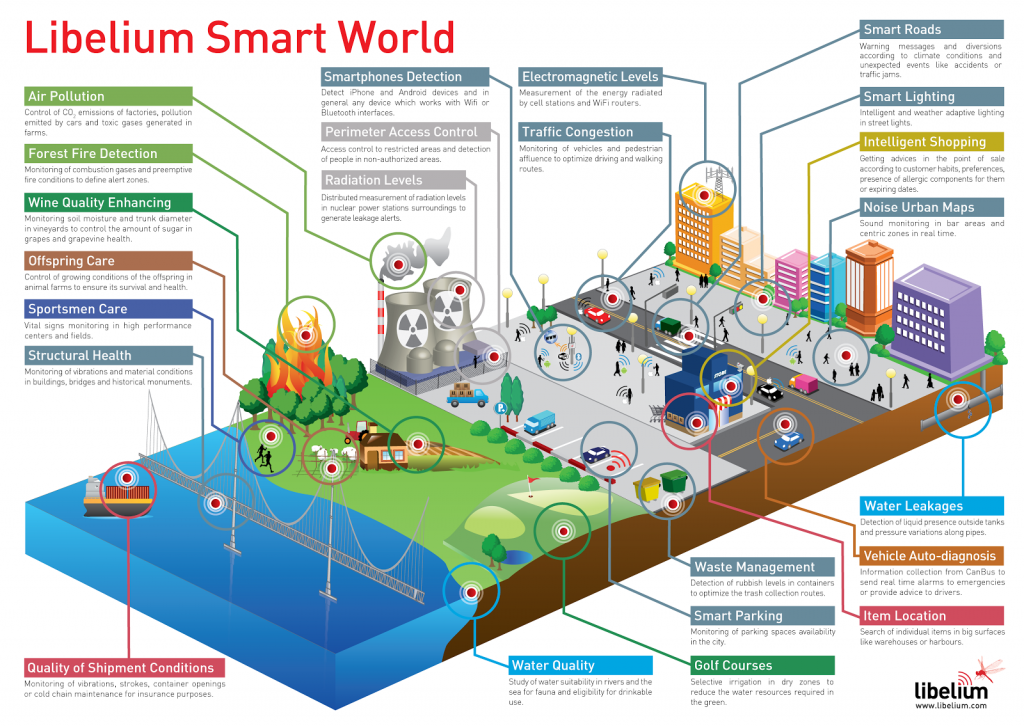
\includegraphics[scale=0.3]{Gambar/smartworld}  
	\caption[Ilustrasi Pemanfaatan \textit{Wireless Sensor Network}]{Ilustrasi Pemanfaatan \textit{Wireless Sensor Network}} 
	\label{fig:smartworld} 
\end{figure} 

		\begin{itemize}
		\item \textbf{Node Sensor}
\begin{itemize}
\item \textbf{Struktur Node Sensor}
\end{itemize}
Setiap node sensor memiliki kemampuan deteksi, komputasi dan komunikasi. Node sensor memiliki lima komponen utama yaitu \textit{controller}, \textit{memory}, \textit{sensor and actuator}, \textit{communication device}, dan \textit{power supply} (Gambar \ref{fig:structure_sensor_node}). Semua komponen akan bekerja secara seimbang dalam melakukan \textit{sensing}, komputasi, komunikasi, dan menjaga penggunaan energi seminimal mungkin. 

\begin{figure} [H]
	\centering  
	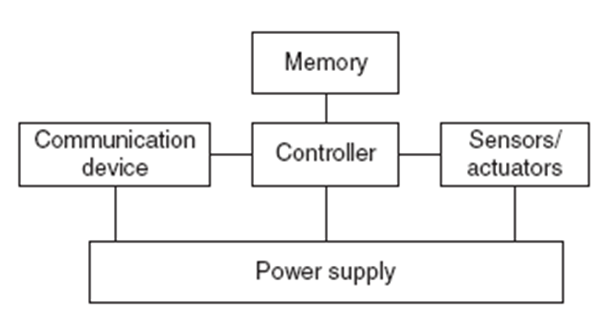
\includegraphics[scale=0.3]{Gambar/structure_sensor_node}  
	\caption[Struktur Node Sensor]{Struktur Node Sensor} 
	\label{fig:structure_sensor_node} 
\end{figure}

\begin{itemize}
\item \textbf{Controller}
\end{itemize}
\textit{Controller} adalah inti utama pada node sensor. \textit{Controller} mengumpulkan data dari sensor dan memproses data tersebut hingga menentukan kapan dan kemana data tersebut dikirim. \textit{Controller} menerima data dari node sensor lain. Pada \textit{controller} biasanya terdapat \textit{microcontroller} atau \textit{microprocessor} yang mengatur dan melakukan komputasi data dari node sensor. \textit{Microcontroller} ini juga dapat mengurangi penggunaan energi dengan adanya \textit{sleep states} yang berarti hanya bagian dari controller saja yang aktif.

Beberapa \textit{microcontroller} yang digunakan dalam \textit{Wireless Sensor Node}:
\begin{itemize}
	\item Intel StrongARM (32-bit RISC, up to 206 MHz)
	\item Texas Instrument MSP 430 (16-bit RISC, up to 4 MHz,RAM 2-10 kB)
	\item Atmel Atmega 128L (8-bit)
\end{itemize}	

\begin{itemize}
\item \textbf{Memory}

\textit{Random Access Memory} (RAM) digunakan untuk menyimpan sementara hasil yang didapat dari sensor. RAM juga menyimpan sementara paket dari node sensor lain. Jika node sensor mati atau energi habis maka data pada RAM ini akan hilang. Data yang hilang saat node sensor mati merupakan salah satu kekurangan dari penggunaan RAM. Untuk itu dalam menyimpan kode program digunakanlah \textit{Read Only Memory} (ROM). ROM ini biasa disebut \textit{Electrically Erasable Programmable Read-Only Memory} (EEPROM) atau \textit{Flash Memory}.
\end{itemize}

\begin{itemize}
\item \textbf{Communication Device}

\textit{Communication Device} digunakan untuk bertukar data antar node sensor. Pada aplikasi WSN, \textit{Radio Frequency(RF)} adalah media komunikasi yang paling relevan untuk saat ini. RF-based mendukung jangkauan yang jauh, memiliki data rate yang tinggi dan tidak perlu saling mengetahui posisi antara penerima dan pengirim.
\\
Pada node sensor dibutuhkan \textit{transmitter} untuk mengirim data dan \textit{receiver} untuk menerima data. Kedua hal ini dapat digabung dan disebut dengan \textit{transceiver}. Tugas \textit{transceiver} adalah mengubah aliran \textit{bit} menjadi gelombang radio. Selain itu \textit{transceiver} juga dapat mengubah gelombang radio menjadi aliran \textit{bit}.
\end{itemize}

\begin{itemize}
\item \textbf{Sensor dan Actuator}

Sensor dan Actuator adalah hal yang penting pada WSN. Tanpa sensor dan actuator maka node sensor tidak berguna dan tidak dapat digunakan. Tabel \ref{tab:sensor} adalah jenis - jenis sensor yang dapat dimiliki node sensor. Sensor dikategorikan menjadi tiga:
\begin{enumerate}
	\item \textbf{Passive, omnidirectional sensors} Sensor ini dapat mengukur kualitas dari lingkungan fisik tempat node sensor tersebut tanpa mengubah lingkungannya. Beberapa sensor dikategori ini \textit{self-powered} yaitu sensor mendapatkan energi yang mereka butuhkan dari lingkungannya. \textit{Omnidirectional} berarti tidak ada arah pada sensor ini. Sensor akan memancarkan sinyalnya ke segala arah. Contoh sensor ini adalah termometer, sensor cahaya, sensor getaran, mikrofon, sensor kelembapan, sensor tekanan udara, sensor deteksi asap, dan lain-lain.
	\item \textbf{Passive, narrow-beam sensors} Sensor ini memiliki sifat yang sama dengan sensor \textit{Passive, omnidirectional sensors} yaitu tidak mengubah lingkungannya. Sensor ini dapat melakukan gerakan dan memiliki arah atau daerah pengukuran. Contoh dari sensor ini adalah kamera yang bisa mengukur sesuai dengan arah yang dituju.
	\item \textbf{Active Sensor} Sensor ini aktif dalam memeriksa lingkungannya. Contoh dari sensor ini adalah sonar, radar atau sensor seismik. Sensor ini menghasilkan gelombang untuk melakukan deteksi.
\end{enumerate}

\textit{Actuator} adalah penerima sinyal dan yang mengubahnya menjadi aksi fisik. \textit{Actuator} jumlahnya beragam seperti sensor.  Contoh aktuator adalah LED, yang mengubah listrik menjadi cahaya dan motor (motor elektrik) juga mengubah listrik menjadi gerakan.

\begin{table} [H]
	\centering 
	\caption{Jenis - jenis sensor yang dapat dimiliki node sensor}
	\label{tab:sensor}
	\begin{tabular}{|p{6cm}|p{9cm}|}
		\toprule
		Sensor & Penggunaan\\

		\midrule
		Accelerometer & Pergerakan 2D \& 3D untuk objek dan manusia  \\
		Acoustic emission sensor & Elastic Waves Generation\\
		Acoustic sensor   & Acoustic pressure vibration\\
		Capacitance sensor  & Solute Concentration\\
		ECG   & Heart Rate\\
		EEG  & Brain Electric Activity\\
		EMG   & Muscle Activity\\
		Electrical/electromagnetic sensor & Electrical Resistivity\\
		Gyroscope  & Angular Velocity \\
		Humidity Sensor   & Mendeteksi Humidity\\
		Infrasonic sensor  &  Gelombang untuk deteksi gempa dan volkanik\\
		Magnetic sensor   & Mendeteksi magnetik\\
		Oximeter   & Tekanan Oxigenation pada darah  \\
		pH sensor  & Tingkat Keasaman\\
		Photo acoustic spectroscopy   & Gas Sensing\\
		Piezoelectric cylinder    &  Gas Velocity\\
		Soil moisture sensor   &  Mengukur tanah\\
		Temperature sensor   & Temperatur \\
		Barometer sensor  &  tekanan air\\
		Passive infrared sensor  & Pergerakan infrared\\
		Seismic sensor   & Pergerakan Seismik (Gempa) \\
		Oxygen sensor  & Oksigen pada darah \\
		Blood flow sensor  & Gelombang ultrasonik pada darah \\

		\bottomrule
		
	\end{tabular} 
\end{table}
\end{itemize}

\begin{itemize}
\item \textbf{Power Supply}

\textit{Power supply} atau sumber energi pada WSN bisa berasal dari dua cara yaitu \textbf{\textit{storing energy}} dan \textbf{\textit{energy scavenging}}. \textit{Storing energy} adalah dengan menggunakan baterai sebagai sumber energinya. Baterai yang digunakan dapat diisi ulang maupun tidak dapat diisi ulang. \textit{Energy scavenging} digunakan saat membuat WSN yang akan digunakan dalam waktu yang lama. Dibutuhkan energi yang bisa dikatakan tidak terbatas. Salah satu cara \textit{energy scavenging} adalah \textit{photovoltaics}. \textit{Photovoltaics} dapat disebut juga \textit{solar cell} yang memanfaatkan cahaya matahari dan mengubahnya menjadi energi sebagai pembangkit daya. Cara lain yang bisa digunakan adalah pemanfaatan angin dan air untuk mengerakan kincir atau turbin yang akan menghasilkan listrik dan digunakan sebagai sumber energi pada node sensor.
\end{itemize}
\end{itemize}
		
		\begin{itemize}
		\item \textbf{Arsitektur dan Topologi}
		
		Pada WSN biasanya akan terdapat banyak node sensor yang disebar pada suatu tempat. Terdapat satu atau lebih \textit{sink node} atau \textit{base station} dalam area sensing tersebut (Gambar~\ref{fig:arsitektur}). \textit{sink node} atau \textit{base station} adalah node sensor yang bertugas untuk mendapatkan data dari node sensor lain. Dalam membuat WSN perlu diperhatikan arsitektur dan topologi yang akan digunakan. Tidak semua topologi jaringan komputer dapat digunakan untuk \textit{Wireless Sensor Network}. 

Ada banyak topologi pada jaringan sensor (\textit{sensor network}). Pada jaringan sensor dengan menggunakan kabel, topologi yang sering digunakan adalah topologi \textit{star}, \textit{line}, atau \textit{bus}. Sedangkan pada jaringan sensor tanpa kabel (WSN), topologi yang biasa digunakan adalah \textit{star}, \textit{tree}, atau \textit{mesh}. 

\begin{itemize}
\item \textbf{Topologi Point-to-Point}

Topologi yang menghubungkan dua titik (Gambar \ref{fig:point2point}). Topologi \textit{Point-to-Point} dibagi menjadi dua yaitu \textit{permanent point-to-point} dan \textit{switched point-to-point}. \textit{Permanent point-to-point} adalah koneksi perangkat keras antara dua titik dan tidak dapat diubah. \textit{Switched point-to-point} adalah koneksi \textit{point-to-point} yang dapat berpindah antara node yang berbeda. 
\begin{figure} [H]
	\centering  
	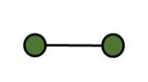
\includegraphics[scale=0.6]{Gambar/point2point}  
	\caption[Topologi Point-to-Point]{Topologi Point-to-Point} 
	\label{fig:point2point} 
\end{figure}

\item \textbf{Topologi Bus}

Topologi Bus seperti pada Gambar \ref{fig:bus} akan terdiri dari node-node dan sebuah jalur. Setiap node akan terhubung dengan saatu jalur yang sama. Untuk mengirim data atau komunikasi akan dilakukan bergantian antar node. Kekurangan dari topologi bus ini adalah jika suatu saat jalur atau bus ini mengalami kerusakan maka setiap node tidak dapat saling berkomunikasi lagi.
\begin{figure} [H]
	\centering  
	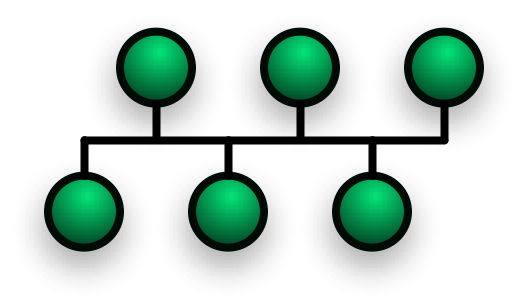
\includegraphics[scale=0.2]{Gambar/bus}  
	\caption[Topologi Bus]{Topologi Bus} 
	\label{fig:bus} 
\end{figure} 

\item \textbf{Topologi Ring}

Pada Topologi \textit{Ring} node akan disusun dengan bentuk melingkar (Gambar \ref{fig:ring}). Setiap node akan terkoneksi dengan dua node lain. Transfer data terjadi dengan cara data akan berjalan dari satu node ke node lain mengikuti jalur melingkar tersebut hingga menemukan node tujuan yang tepat. Topologi ini mudah untuk diimplementasikan tapi kekurangan dari topologi ring adalah saat ada node yang rusak maka perlu biaya lebih untuk memperbaikinya. Biasanya untuk menangani kegagalan komunikasi akibat node yang rusak, akan di atur komunikasi node tidak hanya satu arah tetapi dapat ke arah sebaliknya.
\begin{figure} [H]
	\centering  
	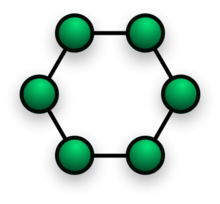
\includegraphics[scale=0.3]{Gambar/ring}  
	\caption[Topologi Ring]{Topologi Ring} 
	\label{fig:ring} 
\end{figure} 

\item \textbf{Topologi Star}

Topologi \textit{Star} terdiri dari satu node yang berada di tengah biasanya berupa \textit{hub} atau \textit{switch} seperti pada Gambar~\ref{fig:star}. Setiap node akan terkoneksi dengan node yang berada di tengah ini. Saat node akan berkomunikasi dengan node lain, node tersebut harus mengirimkan data tersebut ke node yang ada ditengah dahulu dan node yang berada ditengah ini akan meneruskan data tersebut ke node tujuan. Yang paling penting pada topologi ini adalah node yang berada di tengah, karena semua komunikasi harus melalui node tersebut. Jika node tengah mengalami kerusakan maka tidak akan terjadi komunikasi antar node pada jaringan tersebut.
\begin{figure} [H]
	\centering  
	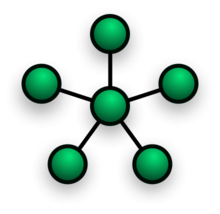
\includegraphics[scale=0.3]{Gambar/star}  
	\caption[Topologi Star]{Topologi Star} 
	\label{fig:star} 
\end{figure} 

\item \textbf{Topologi Tree}

Pada Topologi \textit{Tree} node-node akan disusun secara hierarki dengan satu node yang berada pada level paling atas sebagai \textit{root node} (Gambar~\ref{fig:tree}). \textit{Root node} akan terhubung dengan satu atau lebih node level dibawahnya. Dengan Topologi \textit{Tree} lebih mudah untuk melakukan identifikasi dan meminimalisir kesalahan, namun jika \textit{tree} sudah sangat besar atau \textit{level tree} sudah sangat banyak maka akan sulit untuk melakukan konfigurasi.
\begin{figure} [H]
	\centering  
	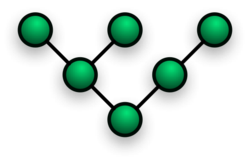
\includegraphics[scale=0.3]{Gambar/tree}  
	\caption[Topologi Tree]{Topologi Tree} 
	\label{fig:tree} 
\end{figure} 

\item \textbf{Topologi Mesh}

Topologi \textit{Mesh} dibagi menjadi dua yaitu \textit{partially connected mesh} dan \textit{fully connected mesh}. Pada \textit{partially connected mesh} (Gambar~\ref{fig:mesh_partial}), node akan terhubung dengan lebih dari satu node. Pada \textit{fully connected mesh} (Gambar~\ref{fig:mesh_fully}), setiap node akan terhubung dengan semua node lain pada jaringan tersebut.
\begin{figure} [H]
	\centering  
	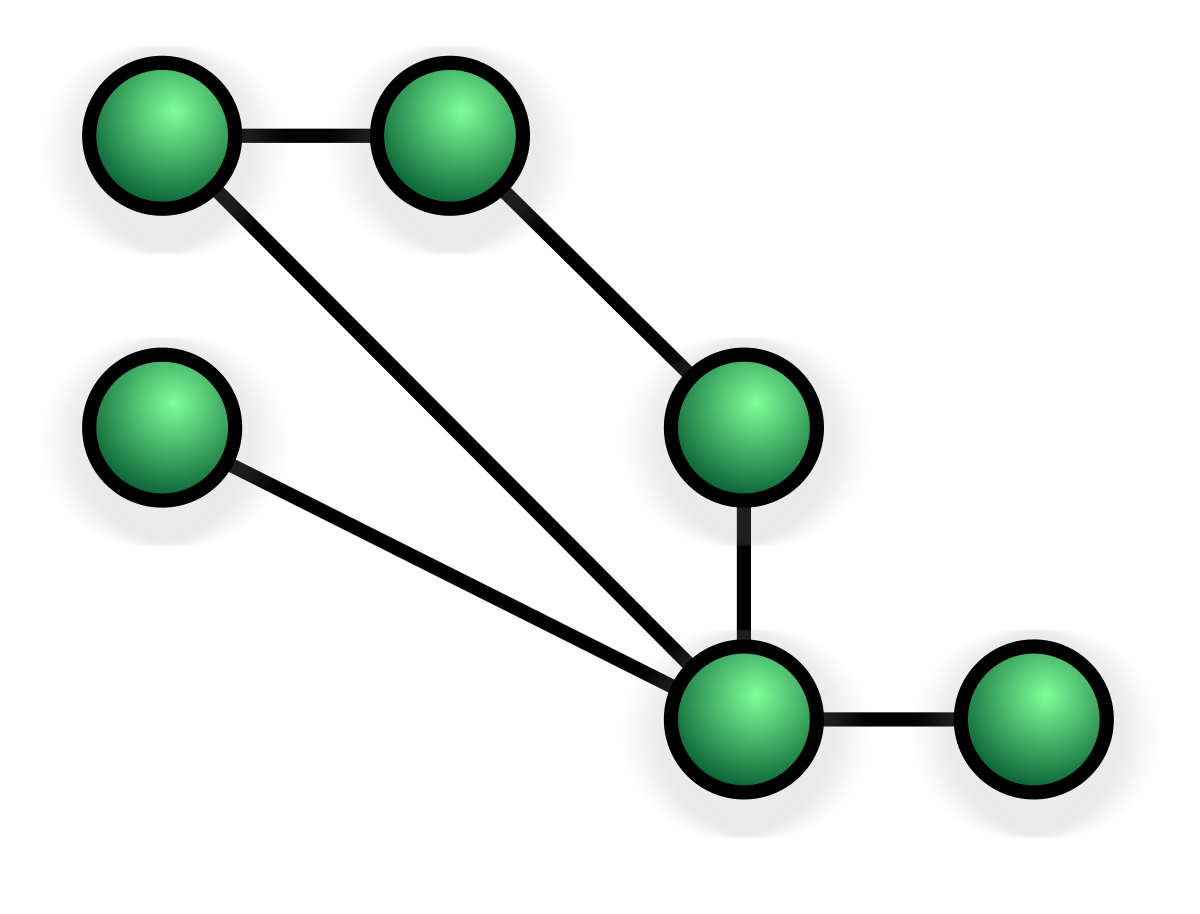
\includegraphics[scale=0.07]{Gambar/mesh_partial}  
	\caption[Topologi Partially Connected Mesh]{Topologi Partially Connected Mesh} 
	\label{fig:mesh_partial} 
\end{figure} 
\begin{figure} [H]
	\centering  
	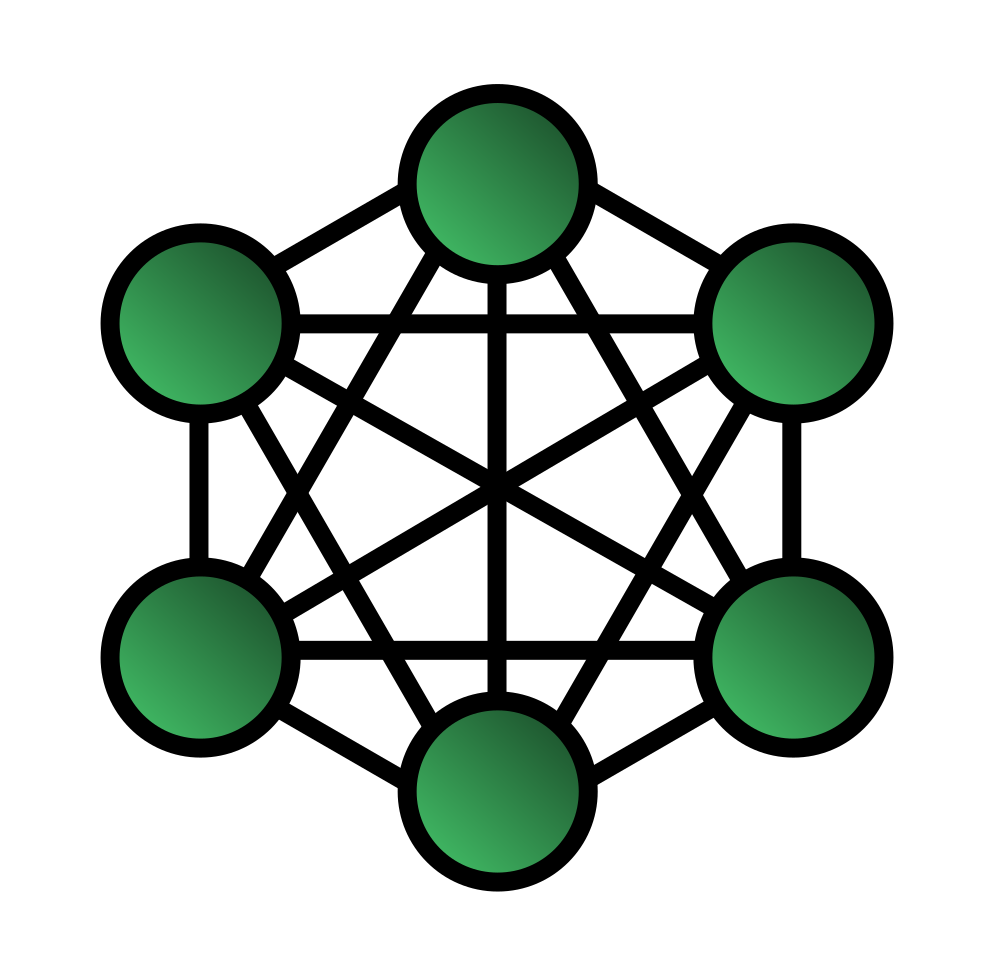
\includegraphics[scale=0.07]{Gambar/mesh_fully}  
	\caption[Topologi Fully Connected Mesh]{Topologi Fully Connected Mesh} 
	\label{fig:mesh_fully} 
\end{figure}

Arsitektur yang biasanya dipakai pada WSN adalah \textbf{arsitektur flat / peer-to-peer} dan \textbf{arsitektur hierarki}. Selain itu dalam membangun WSN perlu juga diperhatikan jalur komunikasi yang digunakan untuk menghubungkan antar node sensor saat transfer data. Untuk area \textit{sensing} yang tidak terlalu luas dan hanya menggunakan sedikit node sensor dapat menggunakan cara komunikasi \textbf{\textit{single hop}}. Sedangkan untuk daerah yang luas dan memerlukan banyak node sensor dapat menggunakan cara komunikasi \textbf{\textit{multi hop}}. 

\begin{figure} [H]
	\centering  
	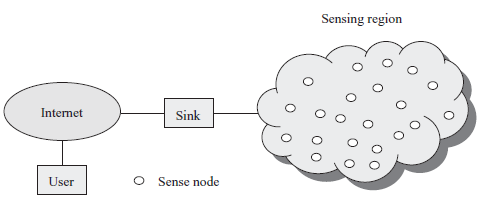
\includegraphics[scale=0.7]{Gambar/arsitektur}  
	\caption[Arsitektur Wireless Sensor Network]{Arsitektur Wireless Sensor Network} 
	\label{fig:arsitektur} 
\end{figure} 

\item \textbf{Single-Hop dan Multi-Hop}

Untuk mengirim data ke \textit{sink node} setiap node sensor dapat menggunakan \textit{single-hop long-distance transmission}. \textit{Single-hop long-distance} ini berarti setiap node sensor akan mengirimkan data ke sink node hanya satu kali lompatan walaupun jarak antara sink node dengan node sensor itu sangat jauh. Dalam jaringan sensor, penggunaan energi paling besar adalah saat melakukan komunikasi dibandingan saat sensing. Penggunaan energi akan semakin bertambah jika jarak sink dan node sensor semakin jauh. Untuk menangani masalah tersebut muncul protokol \textit{multi-hop}.

Pada protokol \textit{multi-hop}, node sensor akan disusun saling berdekatan dan terhubung dengan yang lain. Jadi saat akan berkomunikasi dengan \textit{sink node}, node sensor harus mengirimkan data tersebut ke node sensor tetangganya dan diteruskan hingga sampai ke \textit{sink node}. Karena jarak yang saling berdekatan maka penggunaan energi dapat efektif. \textit{Single-hop} dan \textit{multi-hop} ini dapat digunakan pada topologi flat maupun hierarki sesuai dengan kebutuhan sistem.

\item \textbf{Arsitektur Flat / Peer-to-Peer}

Pada arsitektur flat, setiap node sensor memiliki peran atau \textit{role} yang sama dalam melakukan \textit{sensing}. Secara fungsional hanya terdapat dua macam node sensor pada arsitektur flat, yaitu \textit{source node} dan \textit{sink node}. Untuk mendapatkan data dilakukan dengan cara \textit{sink node} melakukan pengiriman data ke semua node sensor pada area \textit{sensing} dengan cara \textit{flooding} dan hanya node sensor yang sesuai yang akan merespon \textit{sink node}. Setiap node sensor mengirimkan data ke \textit{sink node} dengan \textit{multi hop} dan melalui node tetangganya yang terhubung dengannya untuk meneruskan data (Gambar~\ref{fig:flat}).
% gambar flat
\begin{figure} [H]
	\centering  
	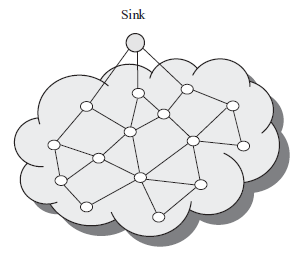
\includegraphics[scale=0.6]{Gambar/flat}  
	\caption[Arsitektur flat pada \textit{Wireless Sensor Network}]{Arsitektur flat pada \textit{Wireless Sensor Network}} 
	\label{fig:flat} 
\end{figure} 

\item \textbf{Arsitektur Hierarki}

Pada arsitektur hierarki, semua node sensor dikelompokan ke dalam cluster-cluster. Terdapat \textit{cluster head} pada setiap cluster. \textit{Cluster head} ini yang mengumpulkan data dari setiap node sensor di bawahnya dan meneruskan data yang telah diterima ke \textit{base station} atau \textit{sink node}. Hal yang perlu diperhatikan pada arsitektur hierarki adalah pemilihan node sensor sebagai \textit{cluster head} dan node sensor yang melakukan sensing. Penggunaan energi yang paling besar dalam WSN ini adalah saat melakukan komunikasi yaitu saat mengirimkan data ke node sensor lain. Maka untuk node sensor yang memiliki energi kecil dapat digunakan untuk \textit{sensing}, karena node sensor ini hanya melakukan komunikasi ke \textit{cluster head}. \textit{Cluster head} harus memiliki energi atau daya yang lebih banyak, karena \textit{cluster head} akan bertugas menerima hasil sensing node sensor di bawahnya dan meneruskan data ke \textit{sink node}. 

Masalah yang utama pada clustering ini adalah pemilihan \textit{cluster head} dan bagaimana cara mengatur setiap cluster. Terdapat beberapa cara untuk membuat clustering ini. Bedasarkan jarak antara \textit{cluster head} dengan cluster member, dapat dibuat clustering dengan \textit{single-hop} atau \textit{multi-hop} seperti pada Gambar~\ref{fig:cluster_single} dan Gambar~\ref{fig:cluster_multi}. Sedangkan jika berdasarkan jumlah \textit{tier} atau tingkat dapat dibangun \textit{clustering single tier} atau \textit{multi tier} (Gambar~\ref{fig:cluster_multitier}).
\begin{figure} [H]
	\centering  
	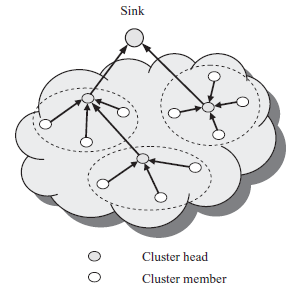
\includegraphics[scale=0.7]{Gambar/cluster_single}  
	\caption[Arsitektur hierarki pada \textit{Wireless Sensor Network} dengan \textit{single hop} terhadap \textit{Cluster Head}]{Arsitektur hierarki pada \textit{Wireless Sensor Network} dengan \textit{single hop} terhadap \textit{Cluster Head}} 
	\label{fig:cluster_single} 
\end{figure} 
\begin{figure} [H]
	\centering  
	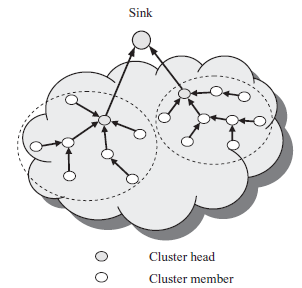
\includegraphics[scale=0.7]{Gambar/cluster_multi}  
	\caption[Arsitektur hierarki pada \textit{Wireless Sensor Network} dengan \textit{multi hop}]{Arsitektur hierarki pada \textit{Wireless Sensor Network} dengan \textit{multi hop}} 
	\label{fig:cluster_multi} 
\end{figure} 
\begin{figure} [H]
	\centering  
	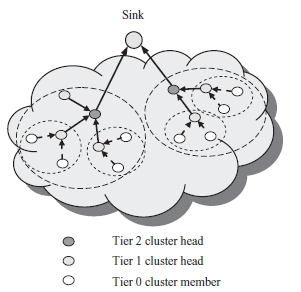
\includegraphics[scale=0.7]{Gambar/cluster_multitier}  
	\caption[Clsutering dengan multi tier]{Clustering dengan multi tier} 
	\label{fig:cluster_multitier} 
\end{figure}
\end{itemize}
		\end{itemize}
		
		\begin{itemize}
		\item \textbf{Sistem Operasi}
		
		Setiap node sensor memerlukan sistem operasi (OS) untuk mengontrol perangkat keras dan perangkat lunak. Sistem operasi tradisional tidak dapat digunakan pada WSN. Pada sistem operasi tradisional digunakan untuk mengatur proses, memori, CPU, dan sistem berkas. Terdapat beberapa hal yang harus ditangani oleh sistem operasi dalam WSN yaitu:
\begin{enumerate}
	\item WSN memerlukan \textit{real-time scheduler}. Data yang didapat harus segera dikirim atau diproses.
	\item Pengaturan memori karena memori pada WSN sangat kecil.
	\item Pengaturan data yang efisien terkait dengan \textit{microprocessor} dan memori yang terbatas
	\item Mendukung kode pemrograman yang efisien dan \textit{reliable} karena dapat terjadi perubahan kode saat implementasi.
	\item Mendukung pengaturan sumber daya untuk menambah waktu hidup dari node sensor dan meningkatkan performa dengan \textit{sleep time} saat tidak ada kegiatan atau \textit{wake up time} saat terdapat interupsi dari lingkungan.
	\item Mendukung antarmuka untuk pemrograman dan antarmuka perangkat lunak. 
\end{enumerate}

Beberapa sistem operasi yang umum digunakan pada WSN antara lain :
\begin{enumerate}
	\item TinyOS
	\item Contiki
	\item LiteOS
	\item PreonVM
\end{enumerate}
		\end{itemize}
		
		\begin{itemize}
		\item \textbf{Protokol Stack pada Wireless Sensor Network}
		\end{itemize}

		\item \textbf{Mempelajari protokol transfer data yang biasa pada \textit{Wireless Sensor Network}.}\\
		{\bf Status :} Ada sejak rencana kerja skripsi.\\
		{\bf Hasil :}

		\item \textbf{Mempelajari library \textit{Wireless Sensor Network} pada Bahasa Pemrograman Java.}\\
		{\bf Status :} Ada sejak rencana kerja skripsi.\\
		{\bf Hasil :}
		
		\item \textbf{Melakukan analisa terhadap protokol transfer yang \textit{reliable} pada \textit{Wireless Sensor Network}}\\
		{\bf Status :} Baru ditambahkan pada semester ini \\
		{\bf Hasil :} 
		
		\item \textbf{Menulis dokumen skripsi 1}\\
		{\bf Status :} Ada sejak rencana kerja skripsi.\\
		{\bf Hasil :} Dokumen skripsi 1 yang telah dibuat adalah Bab 1, Bab 2, dan Bab 3. Bab 1 meliputi Latar Belakang, Rumusan Masalah, Tujuan, Batasan Masalah, Metodologi, dan Sistematika Pembahasan. Bab 2 meliputi studi literatur mengenai \textit{Wireless Sensor Network}, Reliable Data Transfer di WSN, dan PreonVM.

	\end{enumerate}


\section{Pencapaian Rencana Kerja}
Langkah-langkah kerja yang berhasil diselesaikan dalam Skripsi 1 ini adalah sebagai berikut:
\begin{enumerate}
\item Mempelajari permasalahan dari topik skripsi ini.
\item Melakukan studi literartur mengenai \textit{Wireless Sensor Network}.
\item Mempelajari protokol transfer data yang biasa pada \textit{Wireless Sensor Network}.
\item Melakukan analisa terhadap protokol transfer yang \textit{reliable} pada \textit{Wireless Sensor Network}.
\item Menulis dokumen skripsi 1.
\end{enumerate}


\section{Kendala yang Dihadapi}
%TULISKAN BAGIAN INI JIKA DOKUMEN ANDA TIPE A ATAU C
Kendala - kendala yang dihadapi selama mengerjakan skripsi :
\begin{itemize}
	\item Terlalu banyak melakukan prokrastinasi.
	\item Terlalu banyak godaan berupa hiburan (game, film, dll)
\end{itemize}

\vspace{1cm}
\centering Bandung, \tanggal\\
\vspace{2cm} \nama \\ 
\vspace{1cm}

Menyetujui, \\
\ifdefstring{\jumpemb}{2}{
\vspace{1.5cm}
\begin{centering} Menyetujui,\\ \end{centering} \vspace{0.75cm}
\begin{minipage}[b]{0.45\linewidth}
% \centering Bandung, \makebox[0.5cm]{\hrulefill}/\makebox[0.5cm]{\hrulefill}/2013 \\
\vspace{2cm} Nama: \pembA \\ Pembimbing Utama
\end{minipage} \hspace{0.5cm}
\begin{minipage}[b]{0.45\linewidth}
% \centering Bandung, \makebox[0.5cm]{\hrulefill}/\makebox[0.5cm]{\hrulefill}/2013\\
\vspace{2cm} Nama: \pemB \\ Pembimbing Pendamping
\end{minipage}
\vspace{0.5cm}
}{
% \centering Bandung, \makebox[0.5cm]{\hrulefill}/\makebox[0.5cm]{\hrulefill}/2013\\
\vspace{2cm} Nama: \pembA \\ Pembimbing Tunggal
}
\end{document}

